\section{Floating-Point Multiply-Accumulate Unit}
\tableofcontents[currentsection]

\begin{frame}{Standard Floating-Point MAC Design}
	\only<1>{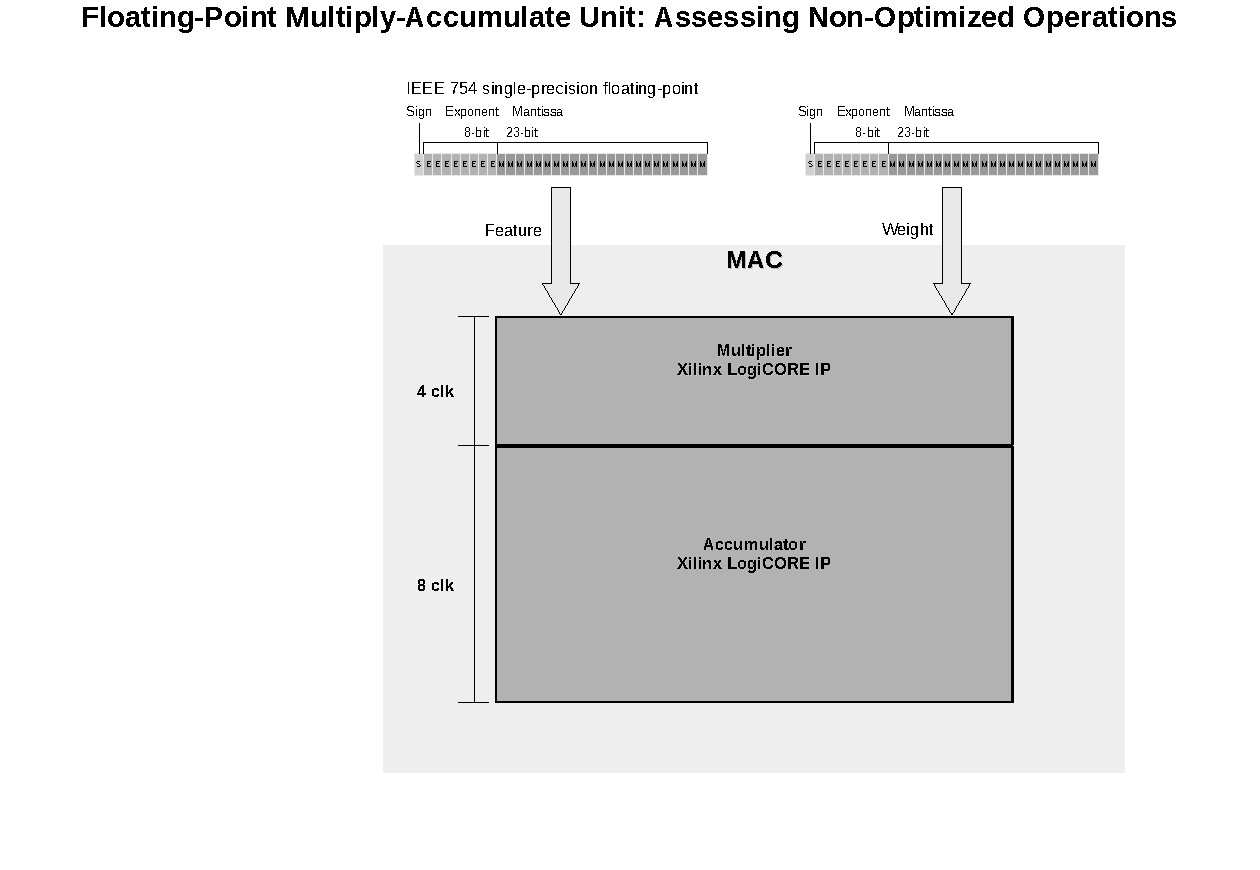
\includegraphics[width=\textwidth]{slides/Methodlogy/mac-fp-1.pdf}}
	\only<2>{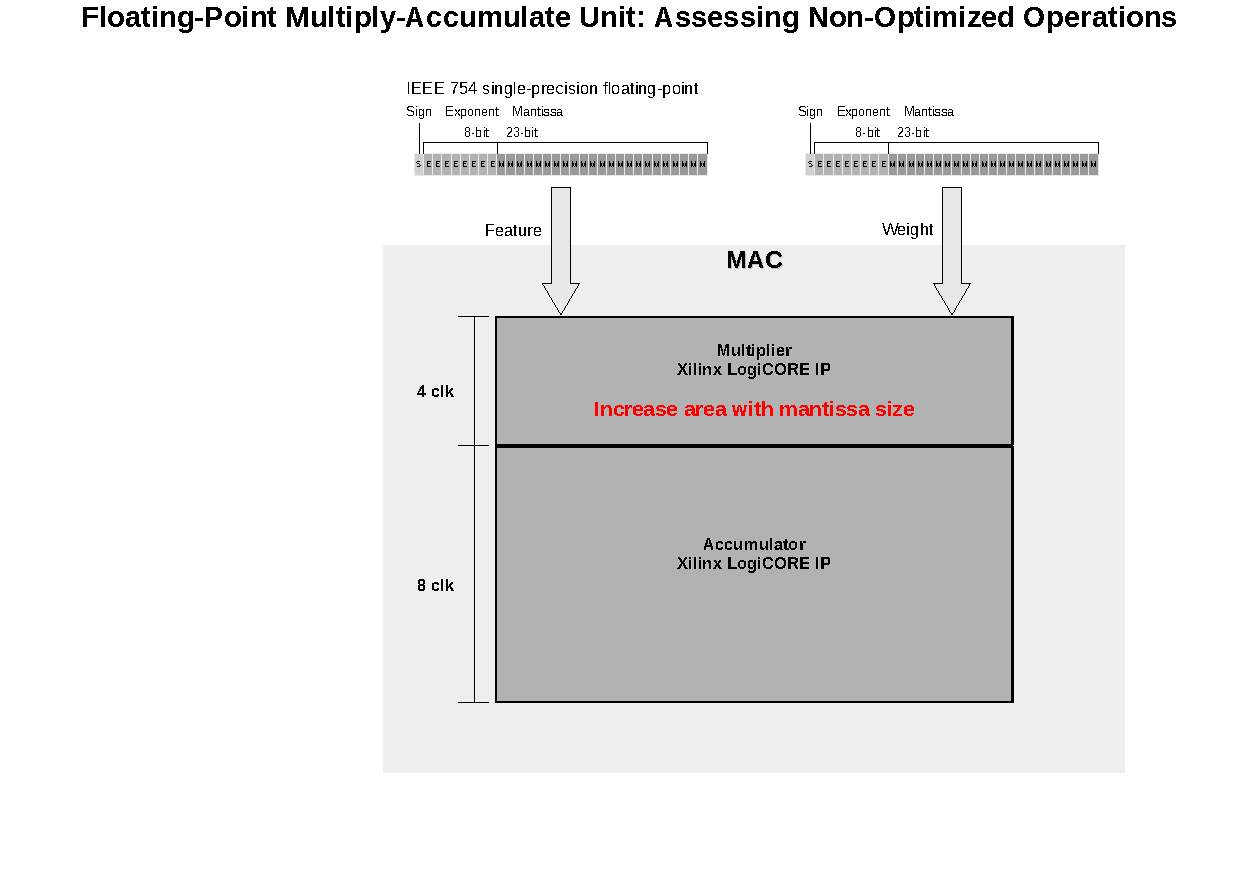
\includegraphics[width=\textwidth]{slides/Methodlogy/mac-fp-2.pdf}}
	\only<3>{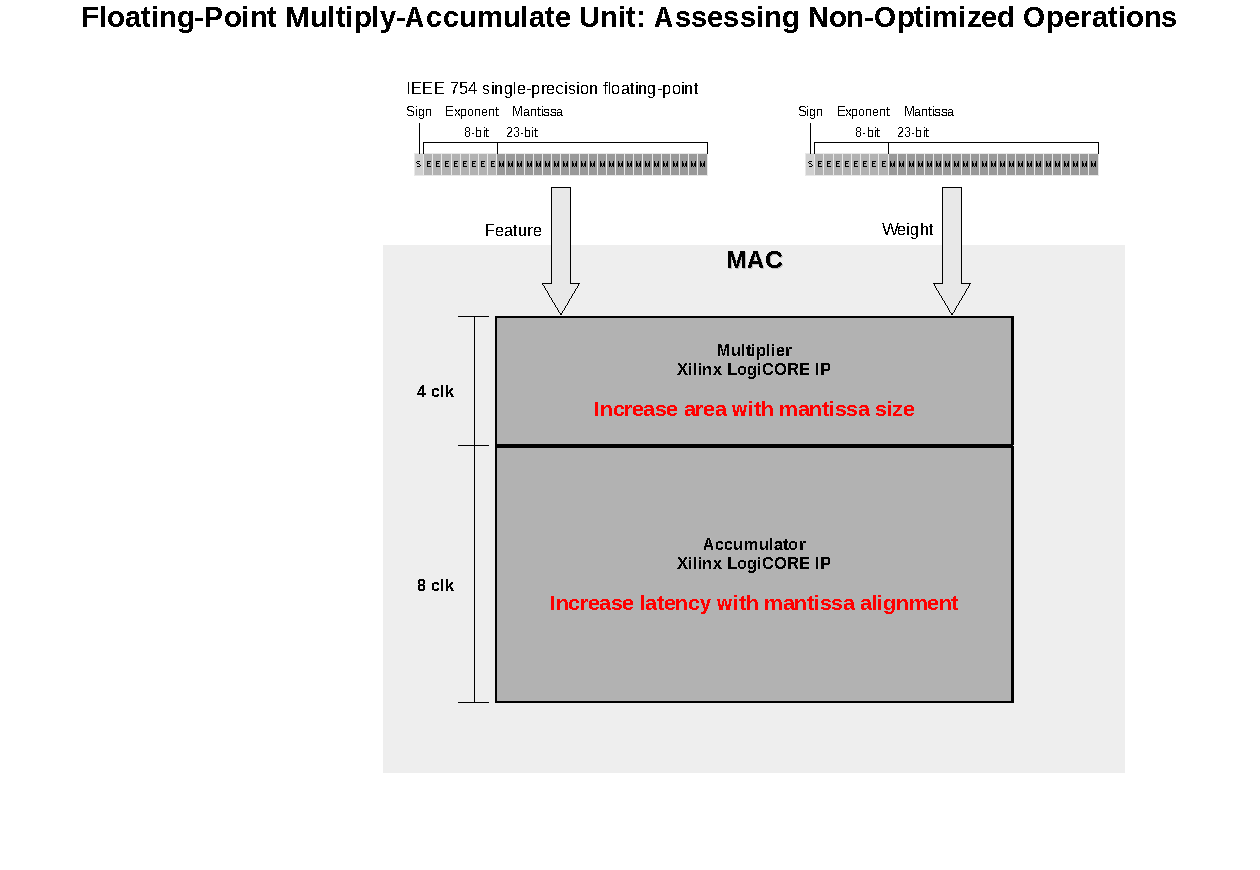
\includegraphics[width=\textwidth]{slides/Methodlogy/mac-fp-3.pdf}}
	\only<4>{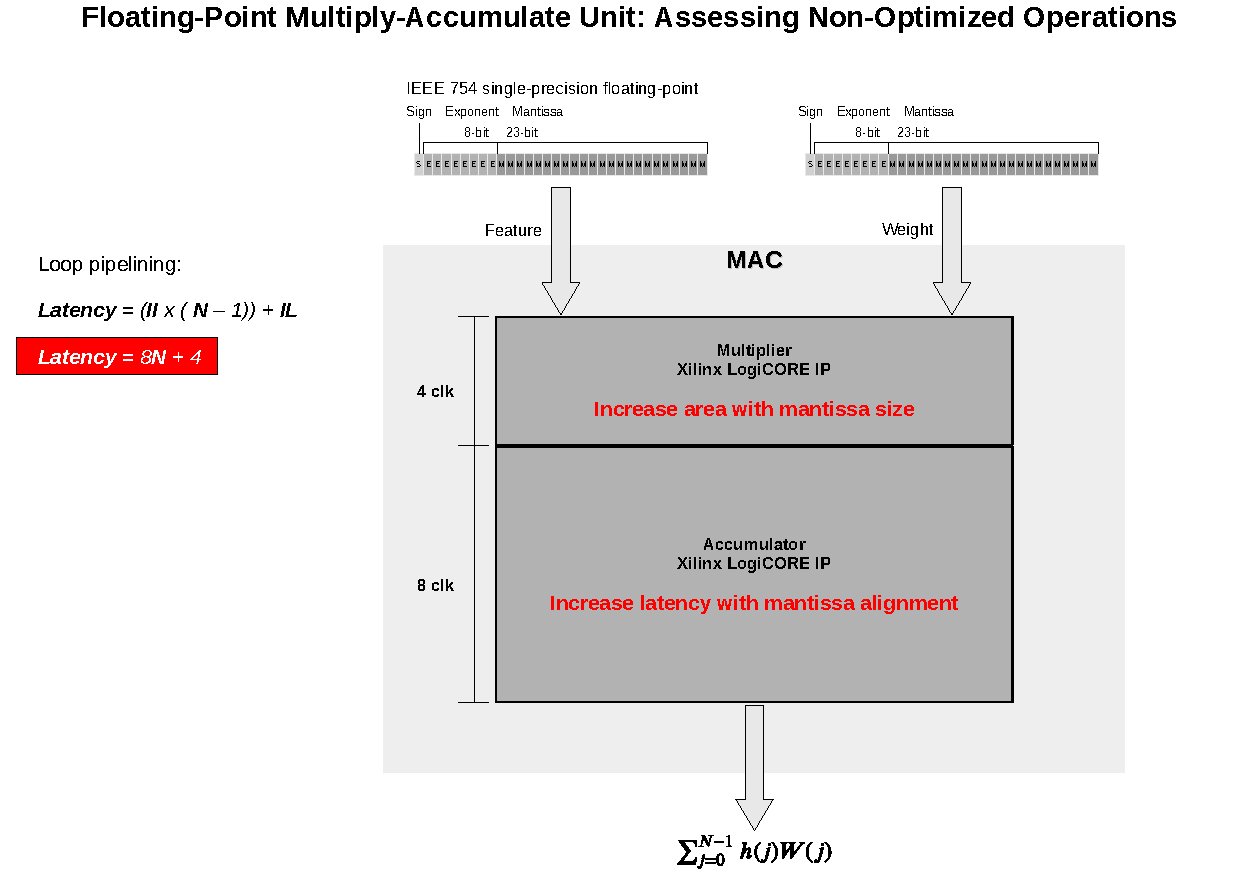
\includegraphics[width=\textwidth]{slides/Methodlogy/mac-fp-4.pdf}}
	\only<5>{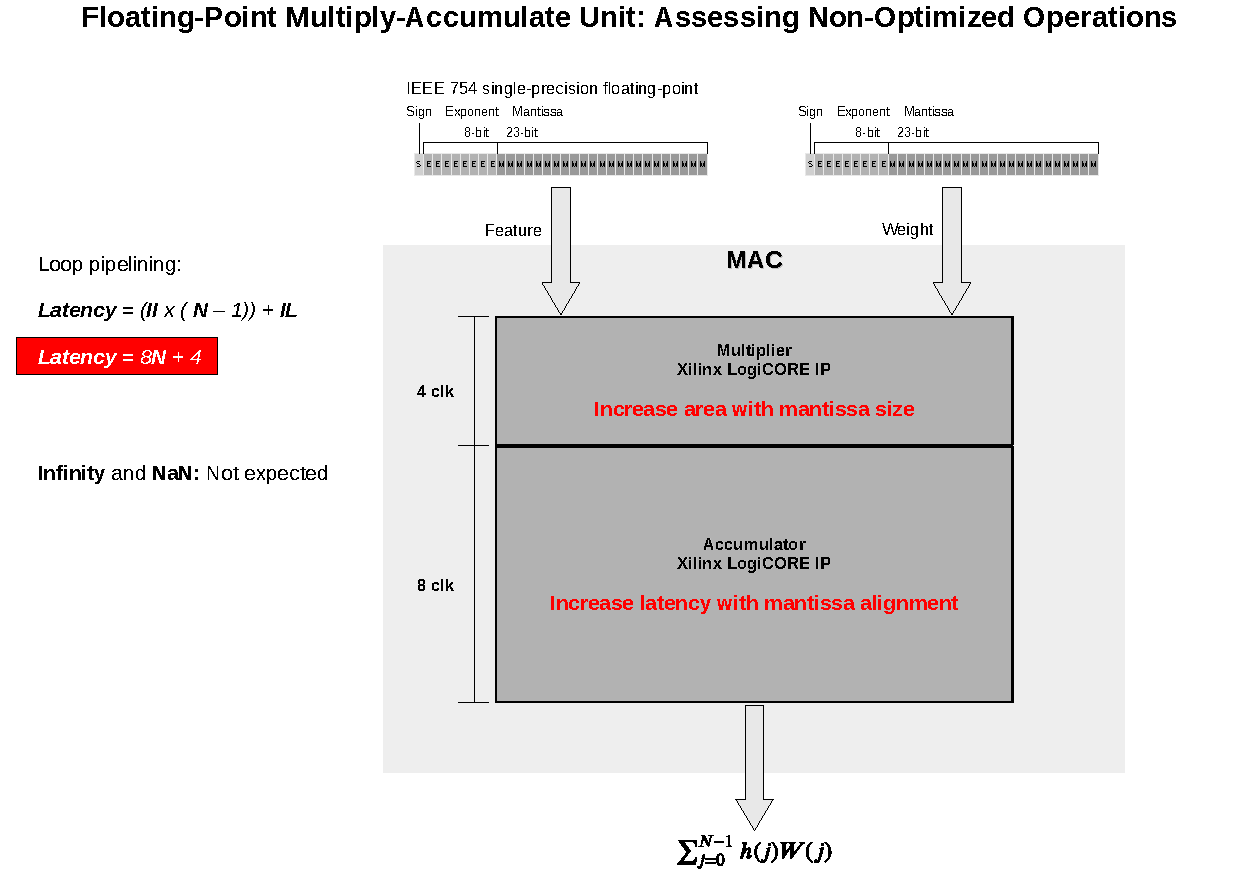
\includegraphics[width=\textwidth]{slides/Methodlogy/mac-fp-5.pdf}}
\end{frame}

\begin{frame}{Custom Floating-Point MAC Designs}
	\only<1>{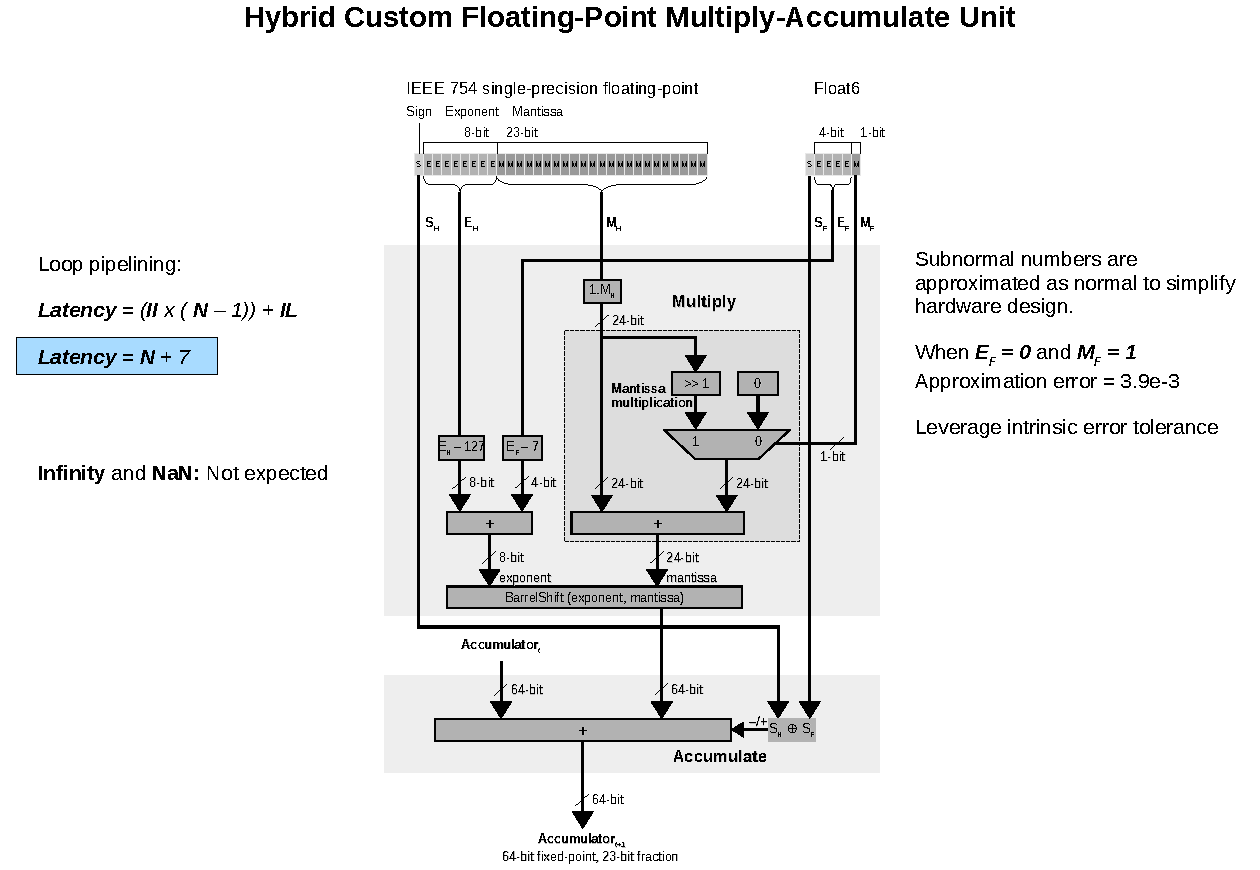
\includegraphics[width=\textwidth]{slides/Methodlogy/mac.pdf}}
	\only<2>{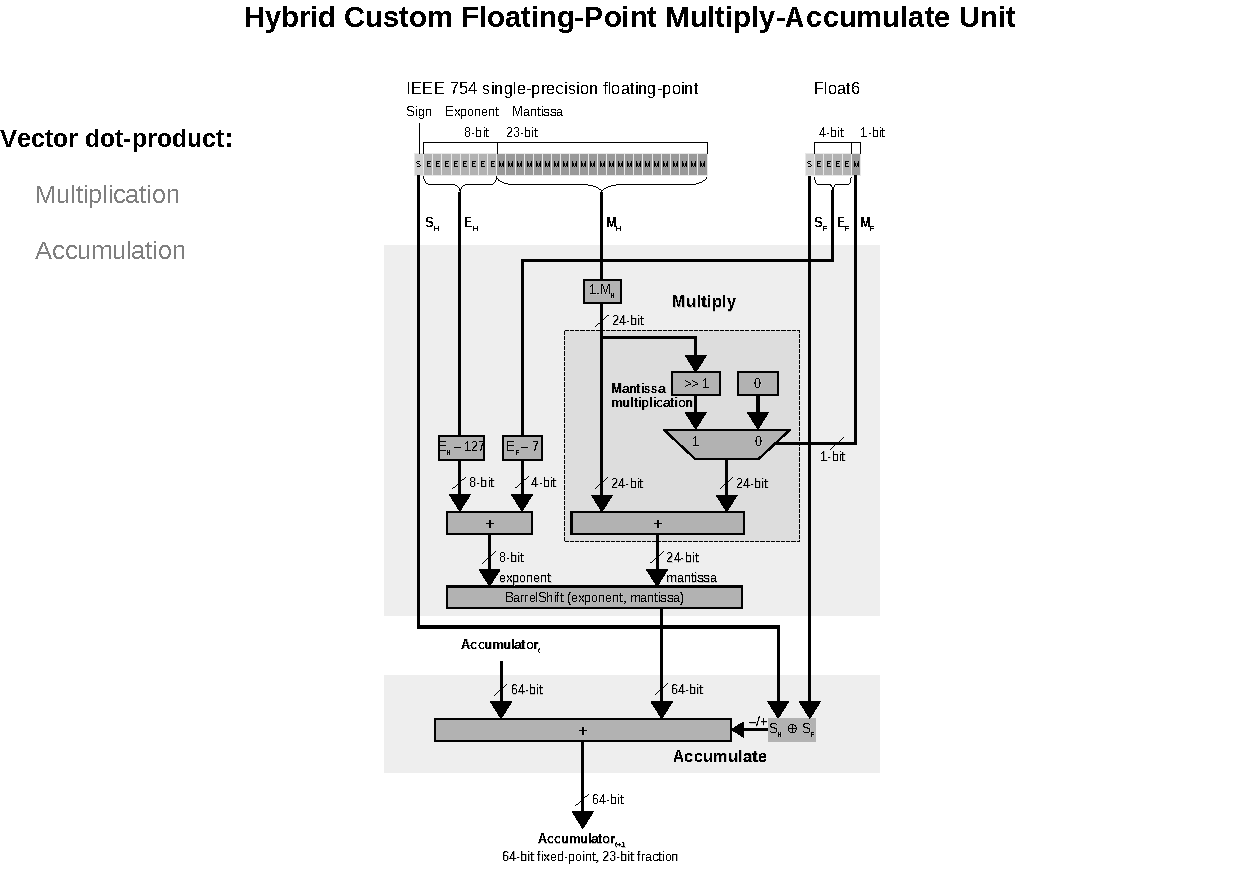
\includegraphics[width=\textwidth]{slides/Methodlogy/mac-2.pdf}}
	\only<3>{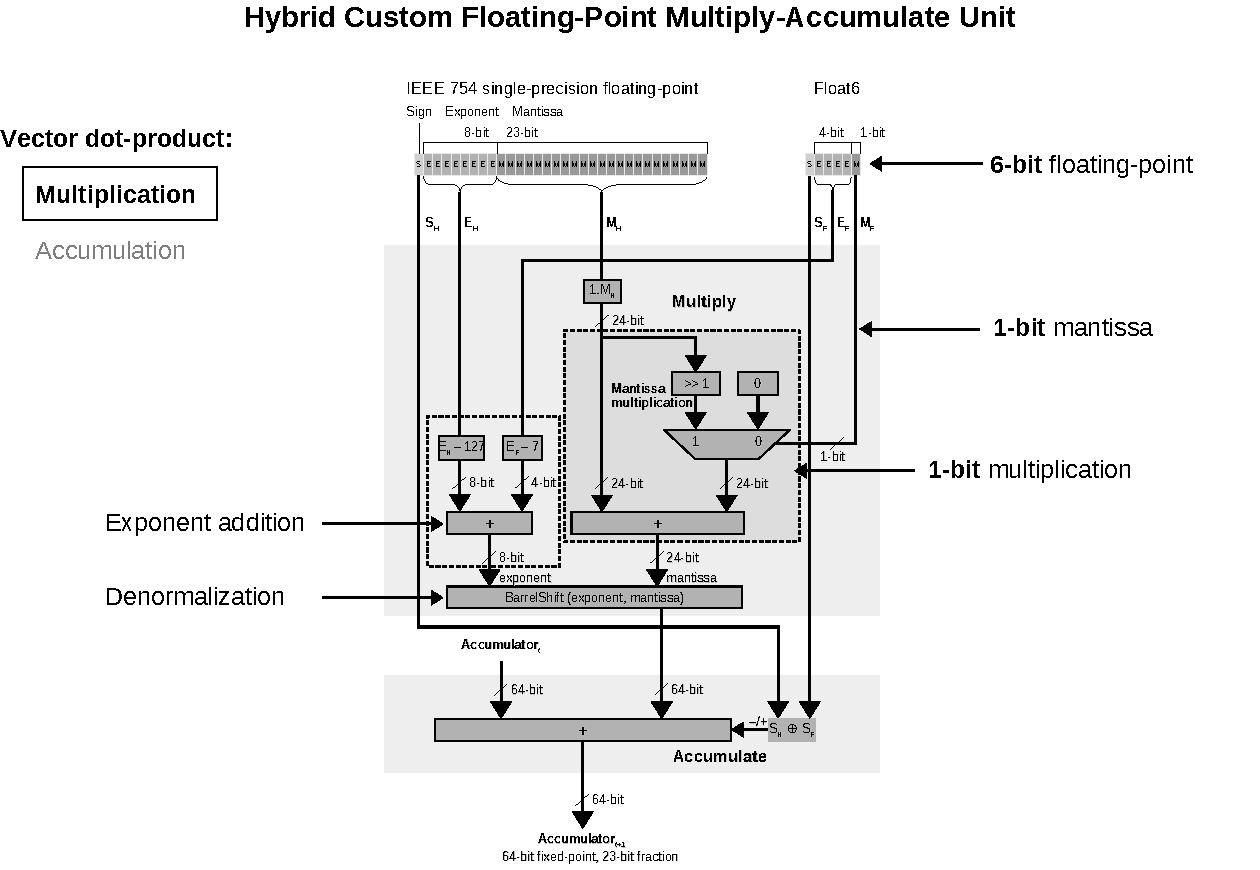
\includegraphics[width=\textwidth]{slides/Methodlogy/mac-3.pdf}}
	\only<4>{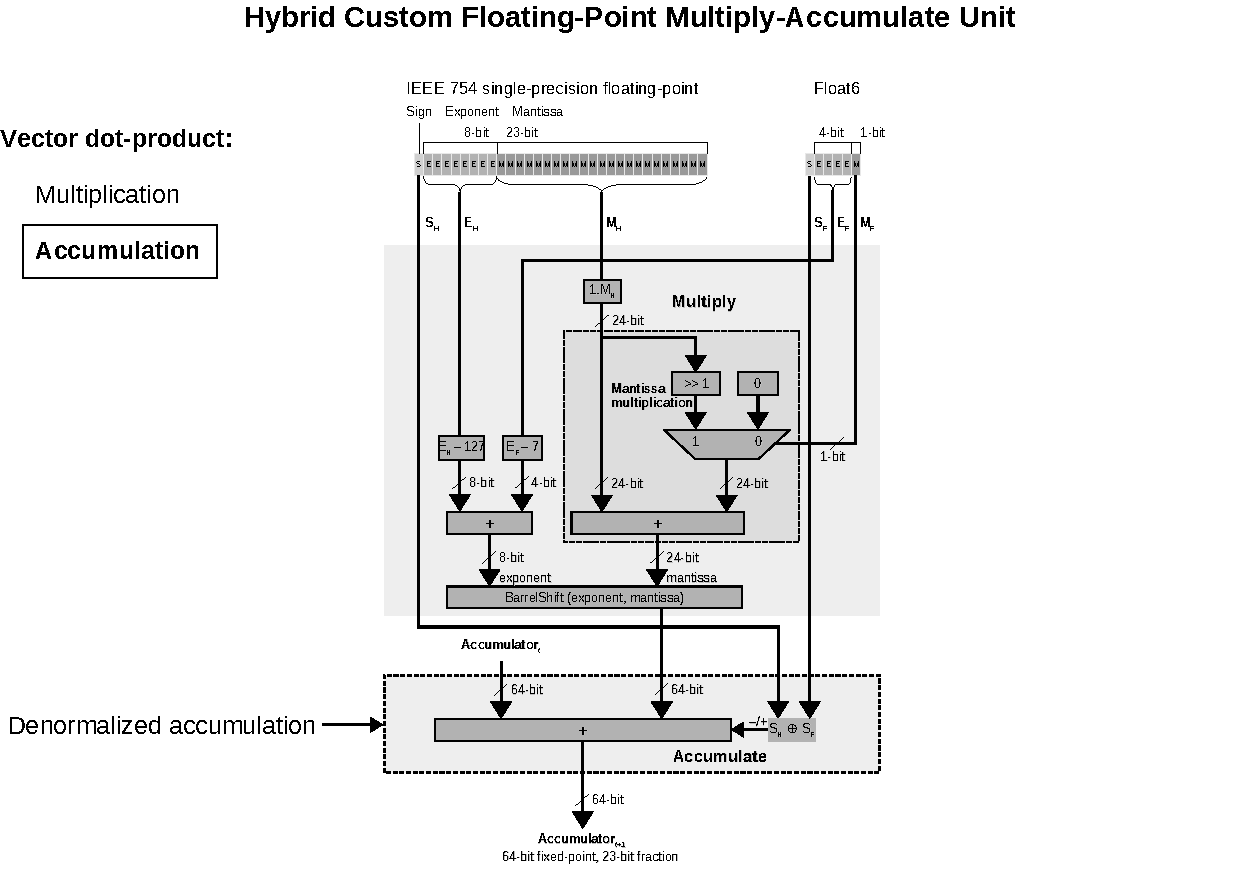
\includegraphics[width=\textwidth]{slides/Methodlogy/mac-4.pdf}}
	\only<5>{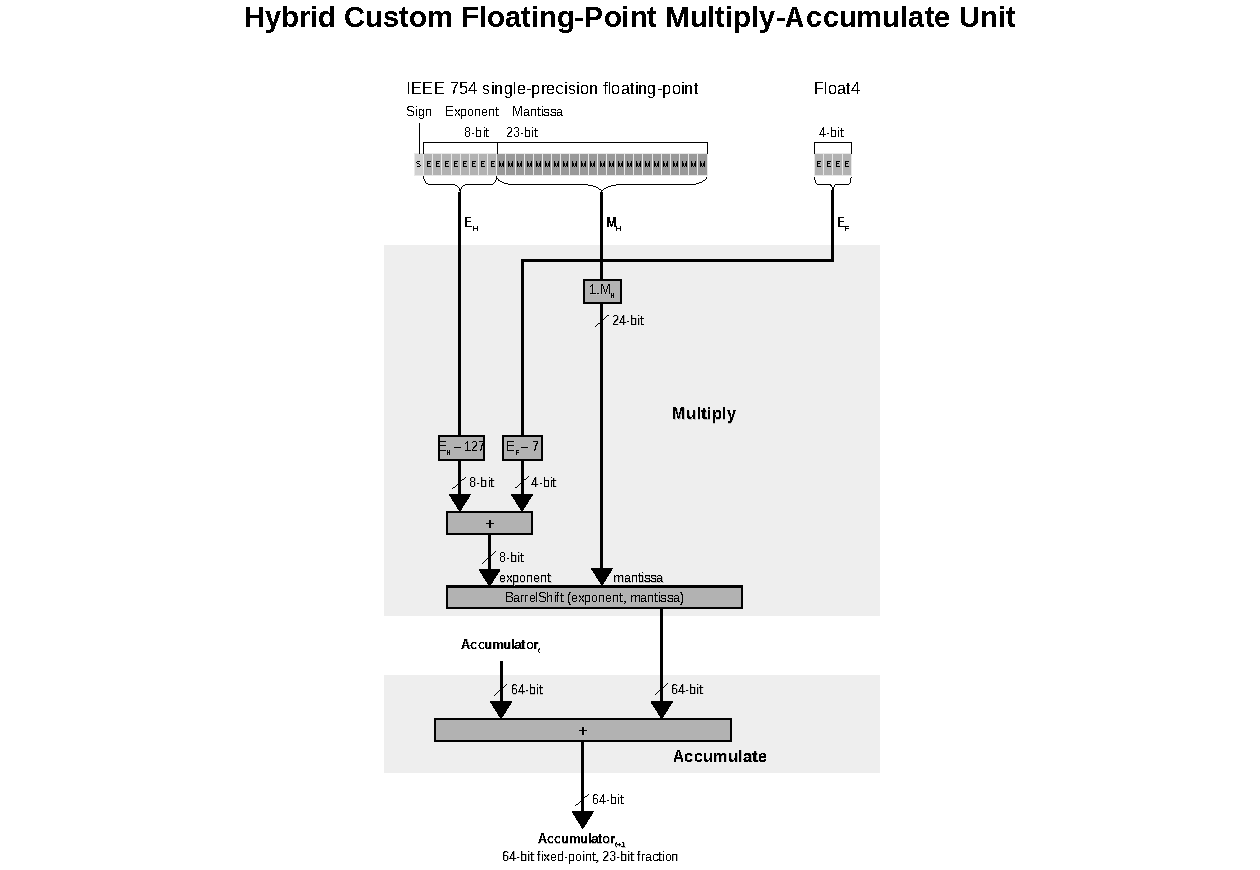
\includegraphics[width=\textwidth]{slides/Methodlogy/mac-5.pdf}}
	\only<6>{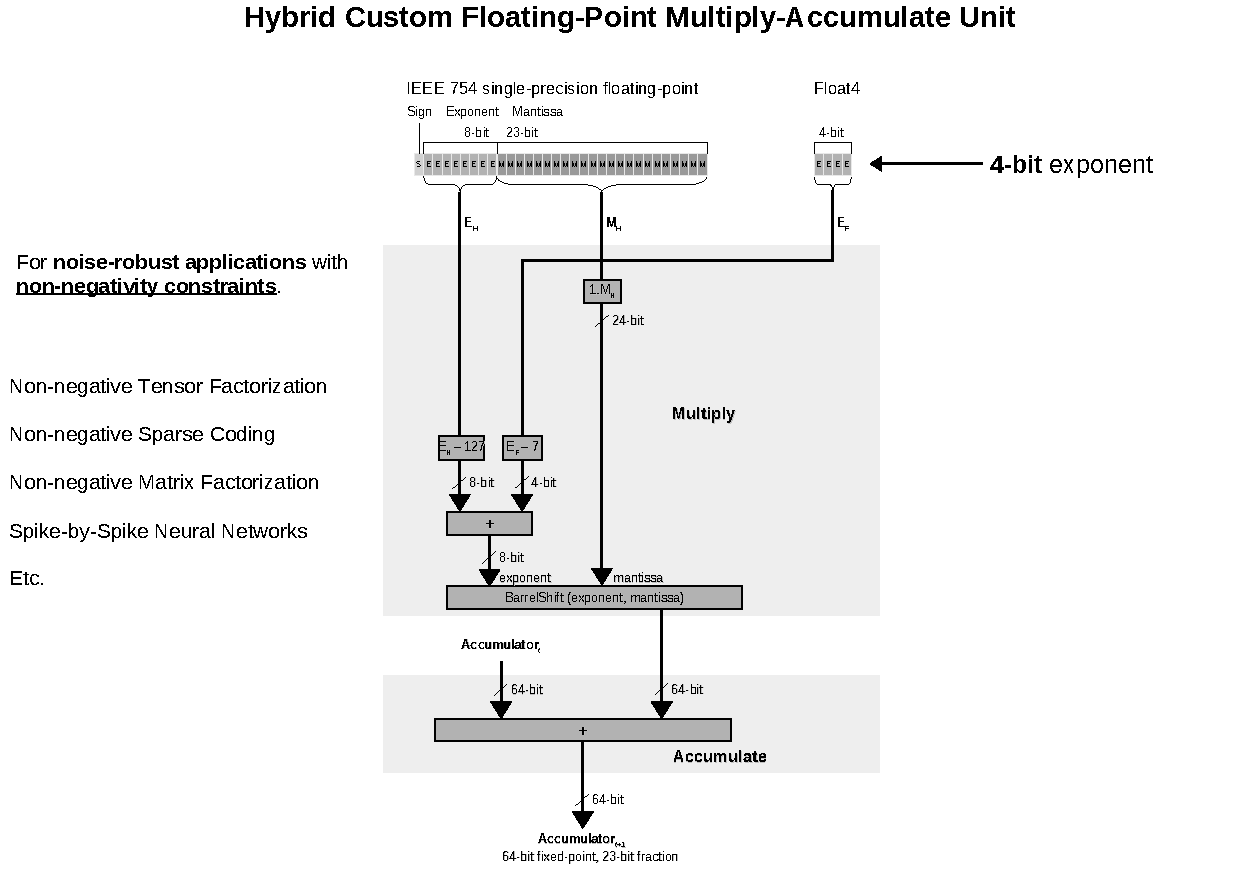
\includegraphics[width=\textwidth]{slides/Methodlogy/mac-6.pdf}}
	%\only<7>{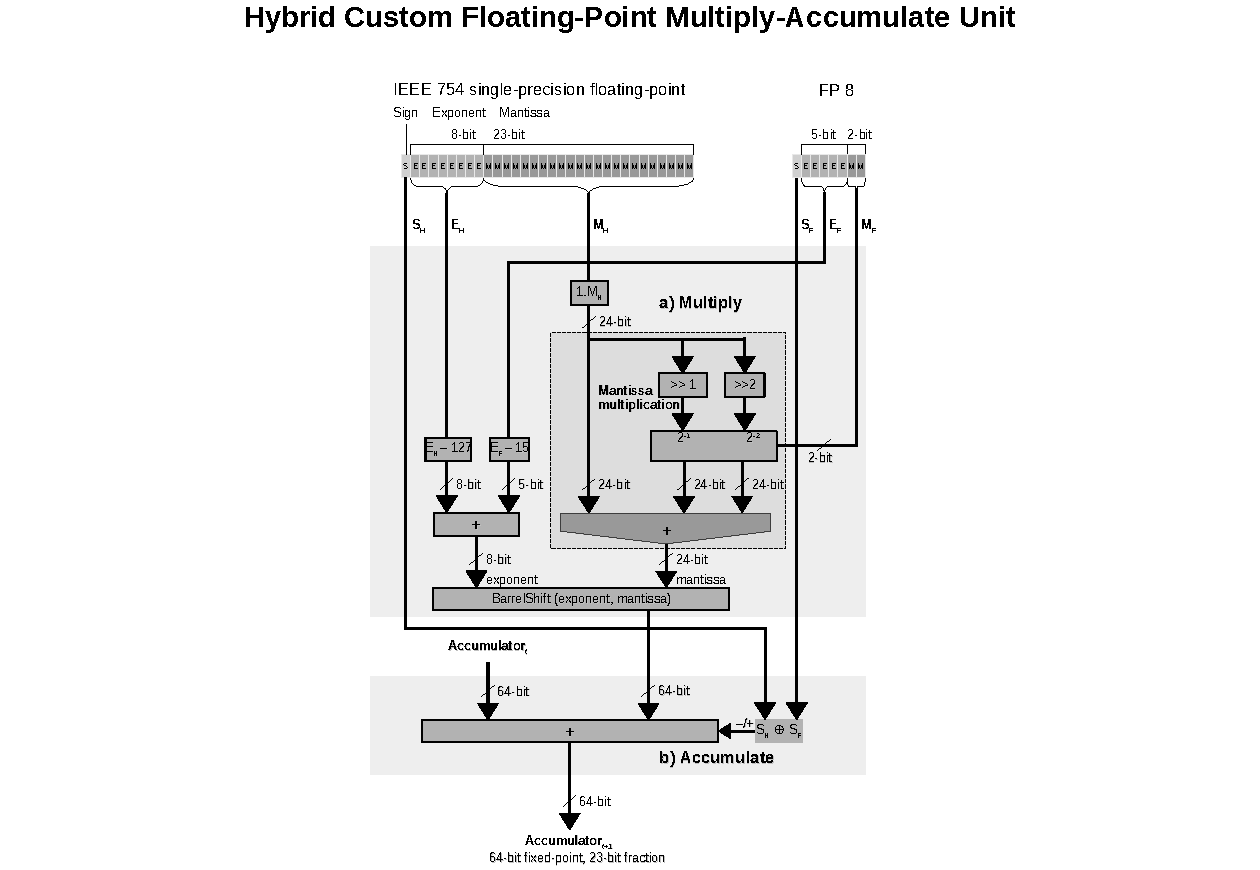
\includegraphics[width=\textwidth]{slides/Methodlogy/mac-7.pdf}}
\end{frame}

%\begin{frame}{Custom Floating-Point Quantization}
%	\only<1>{\centering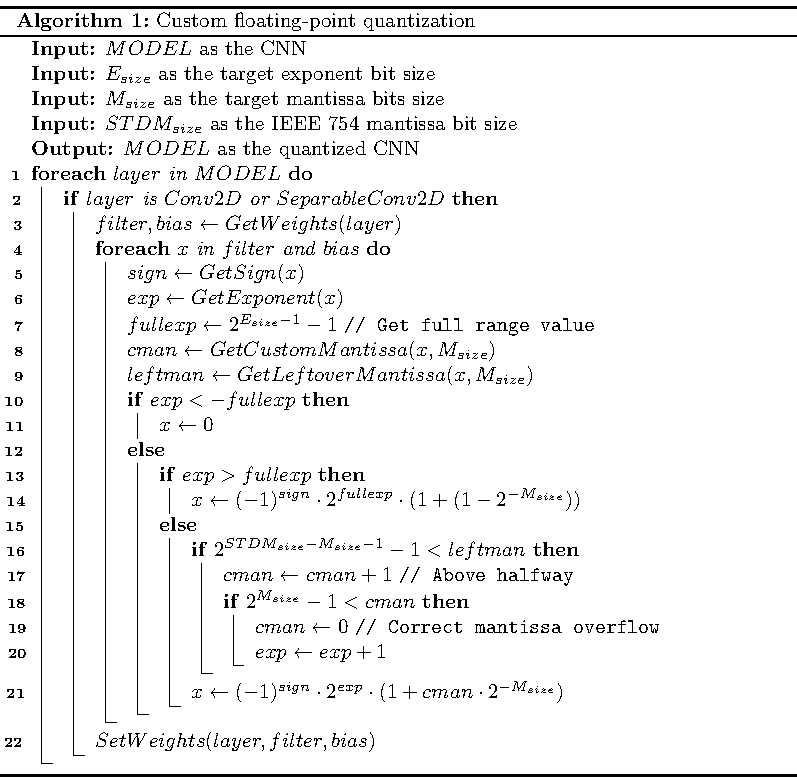
\includegraphics[width=0.7\textwidth]{slides/Methodlogy/qat.pdf}}
%\end{frame}